\chapter{Bacteriología: crecimiento, fisiología y genética}\label{ch:b3:bacteriology}

Una sola célula de \emph{Escherichia coli} en caldo templado se divide
cada veinte minutos. Sin freno, sus descendientes pesarían más que la
Tierra en dos días; de hecho se detienen en cuestión de horas, cuando se
acaba el azúcar, y aguantan semanas en un estado que sobrevive al ayuno.
Una bacteria emparentada, dada una herida y unas horas, se convierte en
cien millones de células y en una fiebre; hace cien años mataba a un
tercio de los pacientes a los que infectaba, y desde 1941 el veneno de un
moho contra ella ha salvado más vidas que ningún otro fármaco --- mientras
que las bacterias, a lo largo de esos mismos ochenta años, han
desarrollado maneras de sortear todos los \omterm{def:b3:bacteriology:antibiotics}{antibióticos} fabricados. Las
bacterias fueron los organismos en los que se demostró por primera vez
que los genes son ADN, en los que se entendió por primera vez la
regulación génica y de los que se tomaron las herramientas del
\cref{ch:b3:genetic-engineering}. Este capítulo las trata como
organismos: su envoltura, la aritmética de su crecimiento en un matraz y
en un cultivo continuo, la manera en que una población detecta su propia
densidad, el tráfico de genes entre células y la química y la evolución de
los \omterm{def:b3:bacteriology:antibiotics}{antibióticos} y la resistencia.

\section{La célula bacteriana}

\begin{definition}[La envoltura]\label{def:b3:bacteriology:envelope}
\index{peptidoglicano}\index{grampositiva}\index{gramnegativa}\index{membrana externa}\index{lipopolisacárido}\index{endospora}
Todas las bacterias salvo unas pocas están encerradas en una pared de
\emph{peptidoglicano}: cadenas alternas de N-acetilglucosamina y de
ácido N-acetilmurámico, entrecruzadas por péptidos cortos en una sola
molécula que rodea la célula y resiste la presión de turgencia --- varias
atmósferas --- del citoplasma. Las bacterias \emph{grampositivas} tienen
una pared gruesa de \qtyrange{20}{80}{nm}, de muchas capas, atravesada por
ácidos teicoicos; las \emph{gramnegativas} tienen una pared fina de una o
dos capas y, por fuera, una segunda bicapa lipídica, la \emph{membrana
externa}, cuya monocapa exterior es \emph{lipopolisacárido} (LPS,
endotoxina --- la molécula que reconoce el sistema inmunitario innato del
\cref{ch:b3:innate-immunity} y que causa el choque séptico), y que
encierra un periplasma. Las porinas de la membrana externa dejan pasar
moléculas pequeñas y excluyen muchos \omterm{def:b3:bacteriology:antibiotics}{antibióticos}. Por fuera puede haber
una cápsula de polisacárido contra los fagocitos, flagelos para nadar
(\cref{ch:b3:cytoskeleton-motility}) y pili para la adhesión y la
\omterm{def:b3:bacteriology:hgt}{conjugación}. Dentro, el cromosoma --- una sola molécula circular de
\qtyrange{1}{10}{Mb} en la mayoría de las especies --- se pliega en un
nucleoide sin membrana, junto a los \omterm{def:b3:genetic-engineering:tools}{plásmidos}. Algunos géneros
(\emph{Bacillus}, \emph{Clostridium}) pueden encerrar una copia del
cromosoma en una cubierta gruesa como \emph{endospora}, deshidratada e
inerte metabólicamente, que sobrevive a la ebullición, a la radiación y a
siglos de sequía y germina cuando vuelven los nutrientes.
\end{definition}

\begin{method}[La tinción de Gram]\label{met:b3:bacteriology:gram}
\index{tinción de Gram}
La prueba más antigua del laboratorio bacteriológico (Gram, 1884) sigue
decidiendo la primera elección de \omterm{def:b3:bacteriology:antibiotics}{antibiótico}. (1) Extiéndase la muestra
y fíjese con calor; (2) tíñase con cristal violeta y después con yodo,
que forma dentro de las células un complejo grande e insoluble con el
colorante; (3) lávese con alcohol: el \omterm{def:b3:bacteriology:envelope}{peptidoglicano} grueso de las
\omterm{def:b3:bacteriology:envelope}{grampositivas}, deshidratado por el alcohol, atrapa el complejo y las
células siguen moradas, mientras que la pared fina de las \omterm{def:b3:bacteriology:envelope}{gramnegativas}
lo deja salir; (4) contratíñase con safranina, que da color rosa a las
\omterm{def:b3:bacteriology:envelope}{gramnegativas}, ya incoloras. La forma y la disposición --- cocos en
racimos (estafilococos) o en cadenas (estreptococos), bacilos, espirales
--- estrechan aún más la identificación, y un coco morado en racimos
procedente de un absceso es un estafilococo antes de que haya crecido
ningún cultivo.
\end{method}

\begin{omfigure}
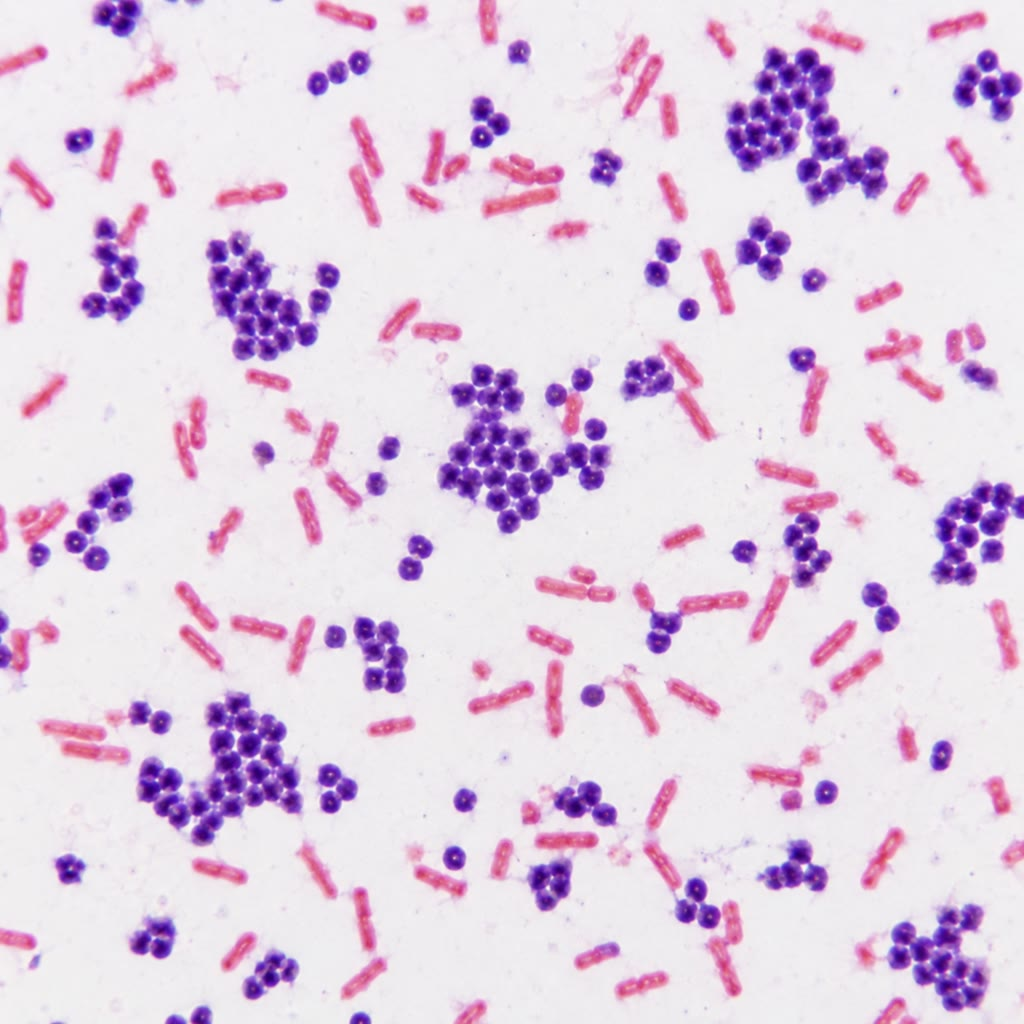
\includegraphics[width=0.36\linewidth]{images/book5/ai/b5-12-gram-stain.jpg}\hspace{0.04\linewidth}
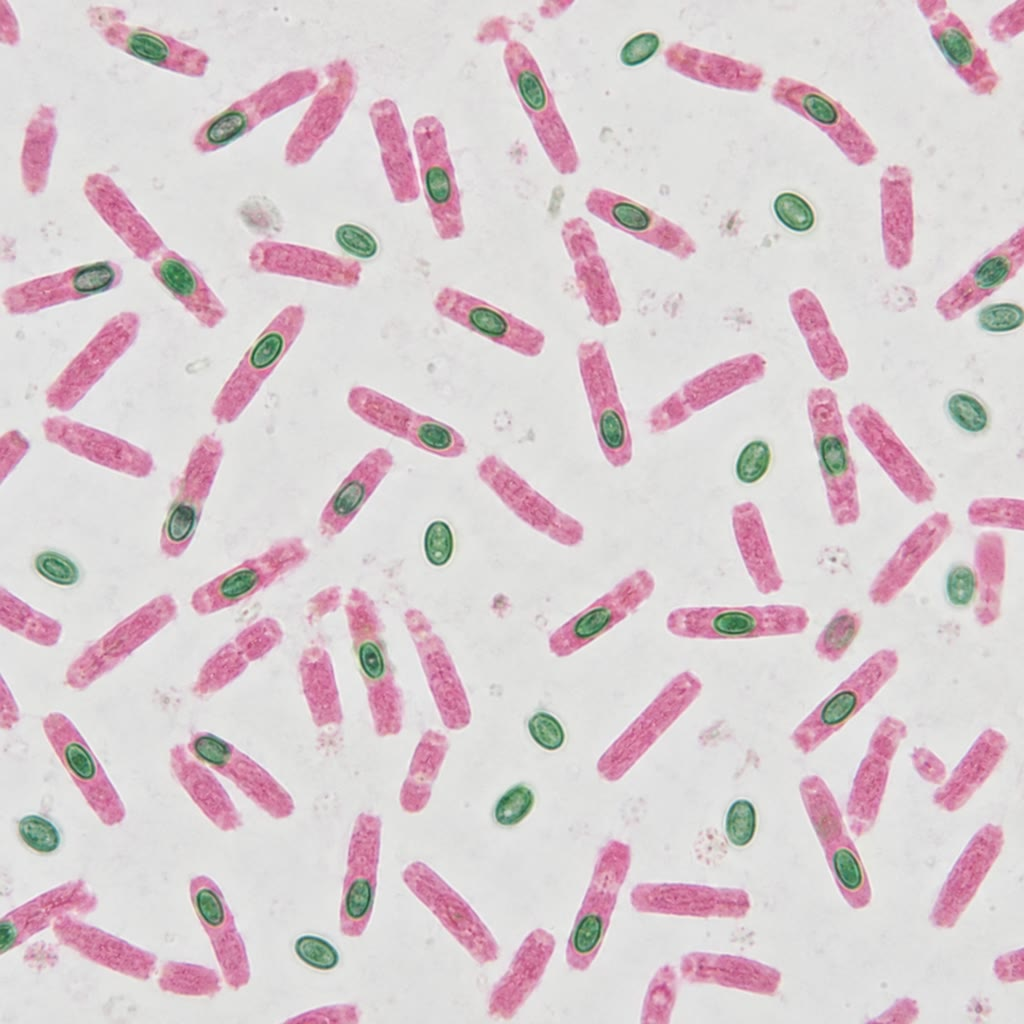
\includegraphics[width=0.36\linewidth]{images/book5/ai/b5-12-endospores.jpg}

{\small Izquierda: una \omterm{met:b3:bacteriology:gram}{tinción de Gram} --- cocos grampositivos morados en
racimos y bacilos gramnegativos rosas. Derecha: células de
\emph{Bacillus} teñidas para las \omterm{def:b3:bacteriology:envelope}{endosporas}, los óvalos verdes brillantes
dentro de células rosas y esporas libres al lado.}
\end{omfigure}

\begin{omfigure}
\begin{tikzpicture}[every node/.style={font=\scriptsize}, >=stealth]
  % Gram-positive
  \begin{scope}
    \fill[omDef!15] (0,0) rectangle (4.5,0.4); \draw[thick, omDef] (0,0) -- (4.5,0); \draw[thick, omDef] (0,0.4) -- (4.5,0.4);
    \fill[omProp!40] (0,0.5) rectangle (4.5,2.0); \foreach \y in {0.7,0.95,1.2,1.45,1.7} \draw[omProp!80!black, thin] (0,\y) -- (4.5,\y);
    \foreach \x in {0.6,1.6,2.6,3.6} \draw[omMeth!70!black, thick] (\x,0.5) -- (\x,2.3);
    \node[below] at (2.25,-0.1) {membrana citoplasmática};
    \node[right, align=left] at (4.6,1.25) {peptidoglicano grueso\\(\qtyrange{20}{80}{nm})}; \node[right, omMeth!70!black] at (4.6,2.2) {ácidos teicoicos};
    \node[above, font=\small\bfseries] at (2.25,2.5) {grampositiva};
  \end{scope}
  % Gram-negative
  \begin{scope}[xshift=8.6cm]
    \fill[omDef!15] (0,0) rectangle (4.5,0.4); \draw[thick, omDef] (0,0) -- (4.5,0); \draw[thick, omDef] (0,0.4) -- (4.5,0.4);
    \fill[omProp!40] (0,0.75) rectangle (4.5,1.05); \draw[omProp!80!black, thin] (0,0.9) -- (4.5,0.9);
    \fill[omDef!15] (0,1.5) rectangle (4.5,1.9); \draw[thick, omDef] (0,1.5) -- (4.5,1.5); \draw[thick, omDef] (0,1.9) -- (4.5,1.9);
    \foreach \x in {0.4,0.9,1.4,1.9,2.4,2.9,3.4,3.9} \draw[omThm, thick] (\x,1.9) -- (\x,2.35);
    \draw[thick, fill=white] (2.0,1.45) rectangle (2.5,1.95); \node[below, font=\tiny] at (2.25,1.45) {porina};
    \node[below] at (2.25,-0.1) {membrana citoplasmática};
    \node[right] at (4.6,0.9) {peptidoglicano fino}; \node[right] at (4.6,1.7) {membrana externa}; \node[right, omThm] at (4.6,2.25) {LPS (endotoxina)};
    \node[right, font=\tiny] at (4.6,1.27) {periplasma};
    \node[above, font=\small\bfseries] at (2.25,2.5) {gramnegativa};
  \end{scope}
\end{tikzpicture}

{\small Las dos envolturas. Las \omterm{def:b3:bacteriology:envelope}{grampositivas} envuelven la membrana en
muchas capas de \omterm{def:b3:bacteriology:envelope}{peptidoglicano}; las \omterm{def:b3:bacteriology:envelope}{gramnegativas} tienen una capa fina y
una \omterm{def:b3:bacteriology:envelope}{membrana externa} de \omterm{def:b3:bacteriology:envelope}{lipopolisacárido} perforada por porinas, que
mantiene fuera muchos \omterm{def:b3:bacteriology:antibiotics}{antibióticos} y fabrica la endotoxina que causa el
choque séptico.}
\end{omfigure}

\section{Crecimiento}

\begin{theorem}[Crecimiento exponencial, ley de Monod y quimiostato]\label{thm:b3:bacteriology:monod}
\index{crecimiento exponencial!bacterias}\index{ecuación de Monod}\index{quimiostato}\index{tasa de dilución}
Una población de $N$ células que se divide con tiempo de generación $T$
crece como $N(t) = N_{0}\,2^{t/T} = N_{0}e^{\mu t}$, con tasa específica
de crecimiento $\mu =
\ln 2/T$. La tasa depende del nutriente limitante $S$ según la \emph{ley
de Monod}
\[
\mu(S) = \mu_{\max}\,\frac{S}{K_{S} + S},
\]
que satura en $\mu_{\max}$ y vale la mitad del máximo en $S = K_{S}$. En
un \emph{quimiostato} --- un recipiente de volumen $V$ al que entra medio
fresco de concentración de nutriente $S_{0}$ a caudal $F$ y del que sale
cultivo al mismo caudal, con \omterm{thm:b3:bacteriology:monod}{tasa de dilución} $D = F/V$ --- el estado
estacionario cumple
\[
\mu(S^{*}) = D,\qquad S^{*} = \frac{K_{S}D}{\mu_{\max} - D},\qquad
X^{*} = Y\,(S_{0} - S^{*}),
\]
donde $X$ es la densidad celular e $Y$ el rendimiento (células producidas
por unidad de nutriente). El experimentador fija la tasa de crecimiento
girando una bomba; el cultivo responde ajustando el nutriente que deja
atrás. Si $D$ supera a $\mu(S_{0})$, las células no pueden seguir el
ritmo y son arrastradas fuera.
\end{theorem}
\begin{proof}
Células: $\mathrm{d}X/\mathrm{d}t = \mu(S)X - DX$, crecimiento menos
salida; en el estado estacionario con $X^{*} > 0$, $\mu(S^{*}) = D$, y al
invertir la ley de Monod se obtiene $S^{*}$. Nutriente:
$\mathrm{d}S/\mathrm{d}t = D(S_{0} -
S) - \mu(S)X/Y$, entrada menos salida menos consumo; en el estado
estacionario, con $\mu = D$, $D(S_{0} - S^{*}) = DX^{*}/Y$, de donde
$X^{*}$. El estado estacionario existe solo si $S^{*} < S_{0}$, es decir,
$D <
\mu(S_{0})$; más allá, el único estado estacionario es $X = 0$, el
arrastre. Estabilidad: si $X$ sube por encima de $X^{*}$ consume más, $S$
cae por debajo de $S^{*}$, $\mu$ cae por debajo de $D$ y $X$ disminuye
--- una retroalimentación negativa a través del nutriente.
\end{proof}

\begin{example}[Un cultivo en números]\label{ex:b3:bacteriology:numbers}
\emph{E.~coli} en medio rico a \qty{37}{\celsius}: $T = \qty{20}{min}$,
$\mu = \qty{2.1}{h^{-1}}$. A partir de una célula, $2^{36}$ al cabo de
doce horas --- $7\times 10^{10}$ células, unos \qty{70}{mg}, que es donde
se detiene un matraz de \qty{100}{mL} por falta de oxígeno y de azúcar;
``la masa de la Tierra en dos días'' son $2^{144}\approx 10^{43}$
células, y la aritmética solo muestra que el crecimiento exponencial
nunca dura. En un quimiostato con glucosa y
$\mu_{\max} = \qty{1.0}{h^{-1}}$, $K_{S} =
\qty{0.01}{g/L}$, $S_{0} = \qty{1}{g/L}$ e $Y = \qty{0.5}{g}$ de células
por gramo de glucosa, una \omterm{thm:b3:bacteriology:monod}{tasa de dilución} de \qty{0.5}{h^{-1}} deja $S^{*}
= 0.01\times 0.5/0.5 = \qty{0.01}{g/L}$ de glucosa y sostiene $X^{*} =
\qty{0.495}{g/L}$ de células, que se dividen cada \qty{83}{min},
indefinidamente. El quimiostato es como se estudia la fisiología a una
tasa de crecimiento fija, y como se corren miles de generaciones de
evolución en una botella.
\end{example}

\begin{omfigure}
\begin{tikzpicture}
\begin{axis}[
  width=6.6cm, height=5.4cm,
  axis x line=bottom, axis y line=left,
  xmin=0, xmax=14, ymin=1e6, ymax=1e10, ymode=log,
  xlabel={horas}, ylabel={células por mL},
  xlabel style={font=\small, at={(axis description cs:0.5,-0.12)}, anchor=north}, ylabel style={font=\small},
  tick label style={font=\scriptsize}, xtick={0,4,8,12},
  clip=false,
]
\addplot[very thick, omDef, domain=0:1.5, samples=2] {1e6};
\addplot[very thick, omDef, domain=1.5:7.5, samples=40] {1e6*2^((x-1.5)/0.5)};
\addplot[very thick, omDef, domain=7.5:12, samples=2] {4.1e9};
\addplot[very thick, omDef, domain=12:14, samples=10] {4.1e9*exp(-0.15*(x-12))};
\node[font=\scriptsize, anchor=south] at (axis cs:0.8,1.2e6) {latencia};
\node[font=\scriptsize, anchor=west] at (axis cs:2.5,3e8) {exponencial: $T = \qty{30}{min}$};
\node[font=\scriptsize, anchor=north] at (axis cs:10,3.5e9) {estacionaria};
\node[font=\scriptsize, anchor=north] at (axis cs:12.8,2.2e9) {muerte};
\end{axis}
\begin{axis}[
  at={(7.8cm,0)}, anchor=south west,
  width=6.6cm, height=5.4cm,
  axis x line=bottom, axis y line=left,
  xmin=0, xmax=0.1, ymin=0, ymax=1.1,
  xlabel={glucosa $S$ (g/L)}, ylabel={$\mu$ (h$^{-1}$)},
  xlabel style={font=\small, at={(axis description cs:0.5,-0.12)}, anchor=north}, ylabel style={font=\small},
  tick label style={font=\scriptsize}, xtick={0,0.01,0.05,0.1}, xticklabels={0,$K_S$,0.05,0.1}, ytick={0,0.5,1},
  clip=false,
]
\addplot[very thick, omThm, domain=0:0.1, samples=60] {x/(0.01+x)};
\addplot[dashed, gray, domain=0:0.1, samples=2] {1};
\addplot[dashed, gray] coordinates {(0.01,0) (0.01,0.5)}; \addplot[dashed, gray] coordinates {(0,0.5) (0.01,0.5)};
\node[font=\scriptsize, omThm, anchor=north west] at (axis cs:0.045,0.6) {Monod: $\mu = \mu_{\max}S/(K_{S}+S)$};
\node[font=\scriptsize, gray, anchor=south east] at (axis cs:0.1,1.01) {$\mu_{\max}$};
\end{axis}
\end{tikzpicture}

{\small Izquierda: un cultivo por lotes --- una latencia mientras se
inducen las enzimas, el crecimiento exponencial, una \omterm{def:b3:bacteriology:phases}{fase estacionaria}
cuando se agota el nutriente y una muerte lenta. Derecha: la ley de
Monod, la tasa de crecimiento frente al nutriente limitante, con $K_{S}$
la concentración a la que el crecimiento es la mitad del máximo.}
\end{omfigure}

\begin{definition}[Fases y estados]\label{def:b3:bacteriology:phases}
\index{fase de latencia}\index{fase estacionaria}\index{esporulación}\index{factor sigma}
En un matraz nuevo (un \emph{cultivo por lotes}) las células primero se
detienen --- la \emph{fase de latencia}, mientras inducen las enzimas que
el medio nuevo exige ---, luego crecen exponencialmente y después paran
cuando se agota un nutriente o se acumula un desecho: la \emph{fase
estacionaria}, en la que las células se encogen, engrosan su envoltura,
condensan su nucleoide en torno a proteínas protectoras, encienden los
genes de estrés a través del factor sigma alternativo RpoS y pueden
sobrevivir meses; sigue una fase de muerte en la que la mayoría se lisa y
unas pocas viven de los restos. Algunas especies responden al ayuno con
un programa de desarrollo: \emph{Bacillus subtilis} se divide de forma
asimétrica y la célula mayor engulle a la menor y construye la espora a
su alrededor, una secuencia de ocho horas controlada por una cascada de
\emph{factores sigma} --- las subunidades que dirigen la ARN-polimerasa
hacia un conjunto de promotores --- que se alterna entre los dos
compartimentos, el primer ejemplo bacteriano de diferenciación y de
señalización de célula a célula a través de una pared.
\end{definition}

\section{Detectarse unas a otras}

\begin{definition}[Percepción de quórum]\label{def:b3:bacteriology:quorum}
\index{percepción de quórum}\index{autoinductor}\index{sistema de dos componentes}
Las bacterias detectan su propia densidad mediante la \emph{percepción de
quórum}: cada célula secreta a velocidad constante una pequeña molécula
señal, un \emph{autoinductor} --- lactonas de homoserina aciladas en las
\omterm{def:b3:bacteriology:envelope}{gramnegativas}, péptidos cortos en las \omterm{def:b3:bacteriology:envelope}{grampositivas} ---; la concentración
en el medio sube con el número de células y, al cruzar un umbral, se une
a un receptor que enciende un conjunto de genes, entre ellos la sintasa
del propio autoinductor (de ahí el nombre). Los genes así controlados son
los que solo compensan en compañía: la luz en \emph{Vibrio fischeri}, los
factores de virulencia en \emph{Staphylococcus aureus} y en
\emph{Pseudomonas aeruginosa}, la matriz de las biopelículas, la
competencia para captar ADN y la eliminación de las vecinas. Casi toda la
detección bacteriana pasa por \emph{sistemas de dos componentes}: una
histidina-quinasa de membrana que detecta un estímulo y fosforila a un
regulador de respuesta citoplasmático, que se une al ADN --- una célula
tiene docenas, para el fosfato, la osmolaridad, el oxígeno y los
autoinductores de otras especies.
\end{definition}

\begin{proof}[Evidencia]
Nealson, Platt y Hastings (1970) cultivaron la bacteria marina luminosa
\emph{Vibrio fischeri} a partir de un inóculo diluido y encontraron que
las células no producían luz hasta alcanzar una densidad de unos $10^{7}$
por mililitro, y entonces se encendían todas a la vez; el medio en el que
había crecido un cultivo denso, esterilizado y añadido a un cultivo
diluido, encendía la luz al instante. Las células estaban contando una
sustancia secretada, no el tiempo ni el nutriente. La sustancia se
identificó como una acil-homoserina-lactona (Eberhard, 1981), y los genes
--- \emph{luxI} para la sintasa, \emph{luxR} para el receptor y el operón
de la luciferasa que controlan --- se clonaron en \emph{E.~coli}, que
entonces brillaba al amontonarse. En el calamar que aloja a la bacteria a
$10^{10}$ por mililitro, el órgano luminoso brilla; en el mar, donde las
bacterias están diluidas, están oscuras y se ahorran el coste.
\end{proof}

\begin{proposition}[Un umbral de densidad]\label{prop:b3:bacteriology:threshold}
\index{percepción de quórum!umbral}
Supóngase que cada una de $N$ células de un volumen $V$ secreta
\omterm{def:b3:bacteriology:quorum}{autoinductor} a razón de $p$ moléculas por segundo, y que la molécula se
pierde (degradada o diluida) con velocidad de primer orden $k$. La
concentración se aproxima a $A^{*} = pN/(kV)$, proporcional a la
densidad celular $N/V$, con constante de tiempo $1/k$; el receptor se enciende
cuando $A^{*}$ alcanza su umbral $A_{\text{umbr}}$, es decir, a la
densidad
\[
\left(\frac{N}{V}\right)_{\text{umbr}} = \frac{k\,A_{\text{umbr}}}{p}.
\]
En un espacio cerrado --- el órgano luminoso de un calamar, un absceso,
el moco de un pulmón --- $k$ es pequeña porque la señal no se la llevan,
de modo que la densidad umbral se alcanza con menos células; en mar
abierto no se alcanza nunca. La célula no mide por tanto su número, sino
su número por unidad del volumen que comparte, que es lo que importa para
cualquier acto cooperativo, y la retroalimentación positiva del
\omterm{def:b3:bacteriology:quorum}{autoinductor} sobre su propia sintasa hace brusco el cambio: en cuanto
unas pocas células cruzan el umbral, su producción adicional empuja al
resto a cruzarlo.
\end{proposition}
\begin{proof}
$\mathrm{d}A/\mathrm{d}t = pN/V - kA$ tiene el estado estacionario $A^{*} =
pN/(kV)$ y relaja hacia él como $e^{-kt}$. Igualando
$A^{*} = A_{\text{umbr}}$ y despejando $N/V$ se obtiene la densidad
umbral.
\end{proof}

\begin{omfigure}
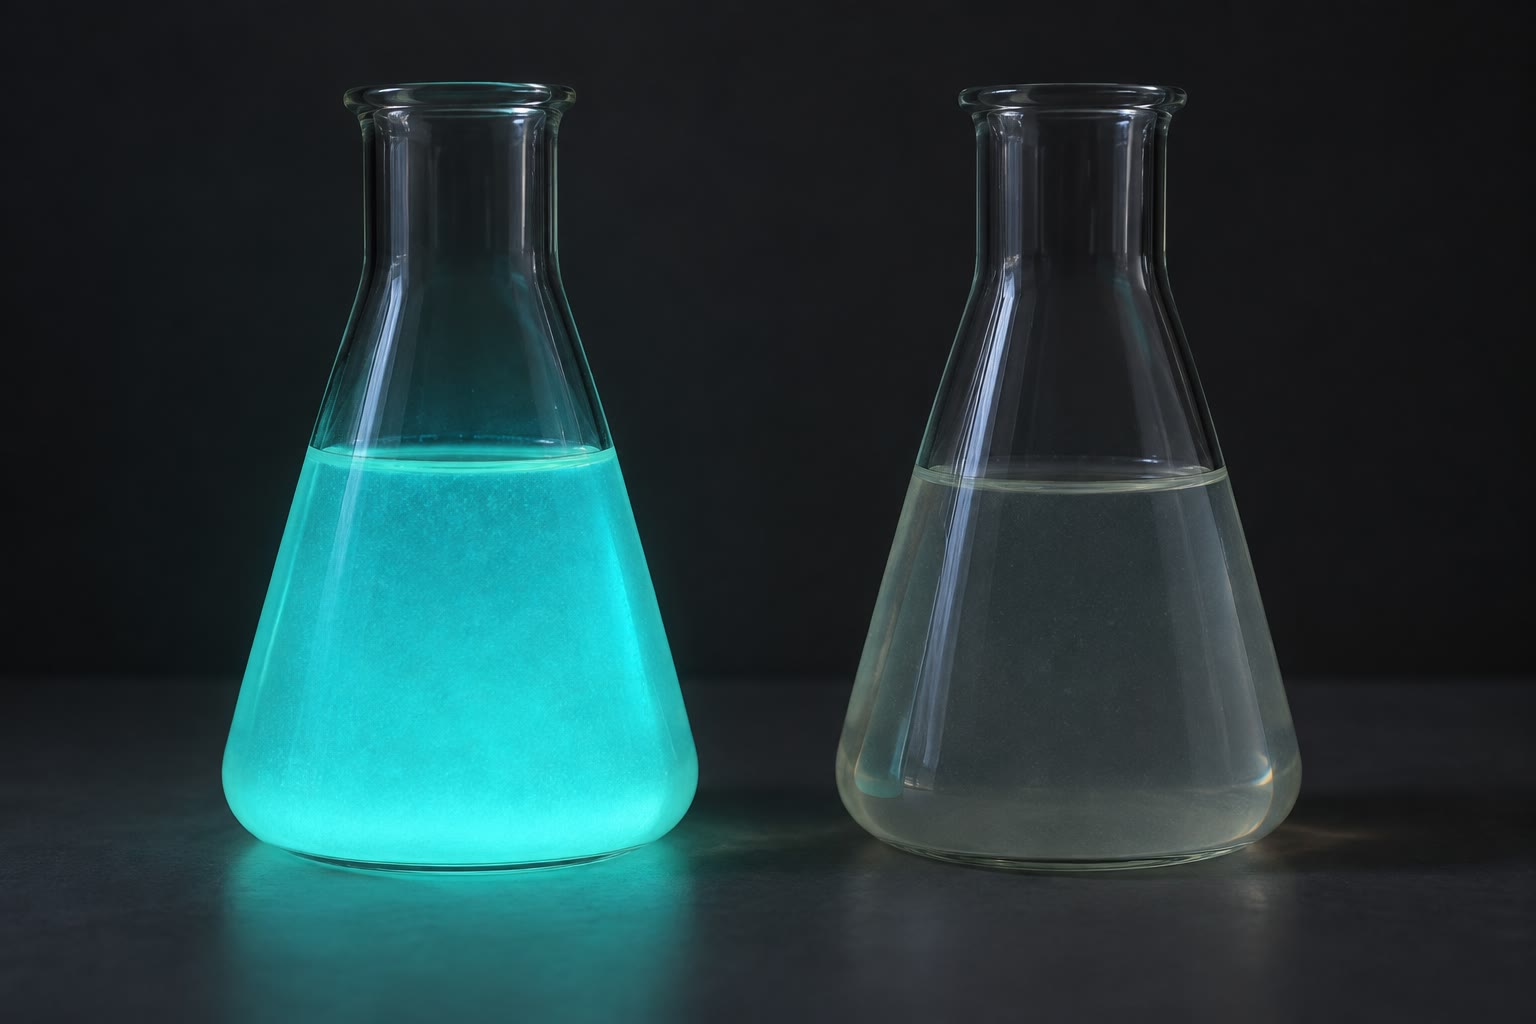
\includegraphics[width=0.46\linewidth]{images/book5/ai/b5-12-quorum-glow.jpg}\hspace{0.04\linewidth}
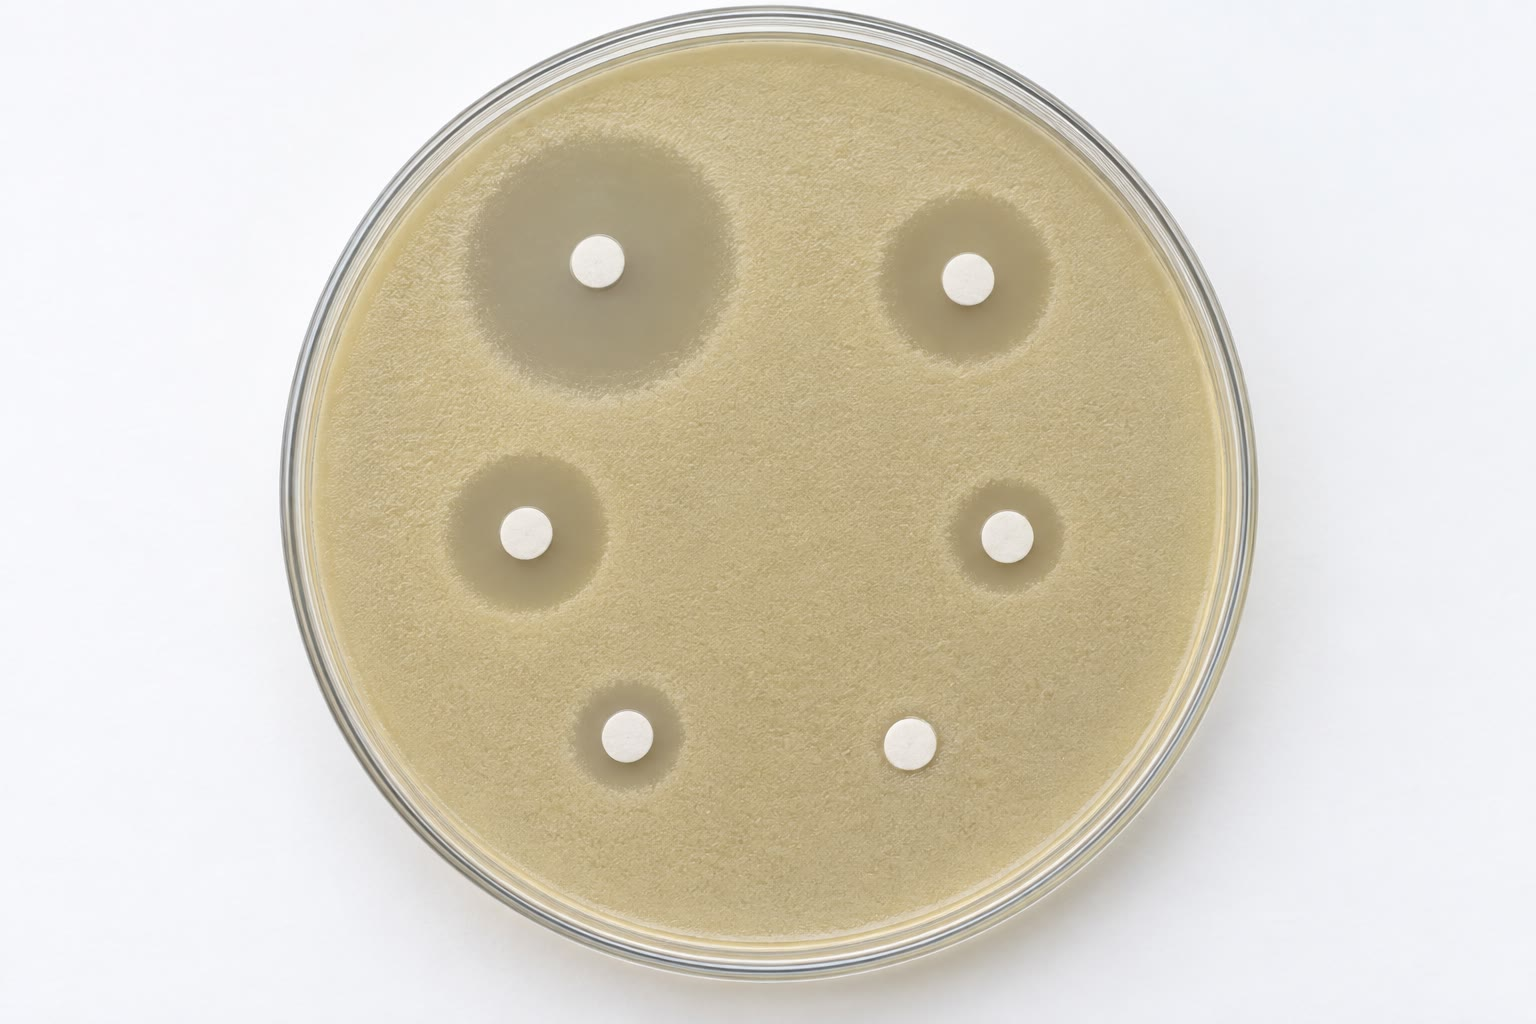
\includegraphics[width=0.46\linewidth]{images/book5/ai/b5-12-antibiotic-disks.jpg}

{\small Izquierda: un cultivo denso de \emph{Vibrio fischeri} brillando,
junto a otro diluido que está oscuro --- las mismas células, por encima y
por debajo de su quórum. Derecha: una prueba de \omterm{met:b3:bacteriology:mic}{difusión en disco}; el
diámetro de cada halo claro mide la sensibilidad de la bacteria al
\omterm{def:b3:bacteriology:antibiotics}{antibiótico} de ese disco, y el disco sin halo marca una resistencia.}
\end{omfigure}

\section{El tráfico de genes}

\begin{definition}[Transferencia horizontal de genes]\label{def:b3:bacteriology:hgt}
\index{transformación}\index{transducción}\index{conjugación}\index{plásmido!de resistencia}\index{elemento genético móvil}\index{pangenoma}
Las bacterias se reproducen de forma clonal pero intercambian genes por
tres rutas. La \emph{transformación}: la captación de ADN desnudo del
ambiente por una célula competente --- la ruta por la que los neumococos
de Griffith adquirieron su cápsula y con la que Avery demostró que el
principio transformante era ADN (1944). La \emph{transducción}: un fago
que empaqueta un trozo de ADN del hospedador y lo inyecta en el siguiente
(\cref{ch:b3:virology}). La \emph{conjugación}: la transferencia de un
\omterm{def:b3:genetic-engineering:tools}{plásmido} a través de un pilus y de un puente de apareamiento desde una
donadora que lo lleva hasta una receptora, demostrada por Lederberg y
Tatum (1946) con cepas auxótrofas de \emph{E.~coli} que producían
recombinantes prototrofas solo al mezclarse. Los \omterm{def:b3:genetic-engineering:tools}{plásmidos} conjugativos
llevan sus propios genes de transferencia; muchos llevan además genes de
resistencia, a menudo agrupados en \emph{integrones} y flanqueados por
transposones, de modo que un solo apareamiento puede transferir la
resistencia a cinco \omterm{def:b3:bacteriology:antibiotics}{antibióticos} de una vez, entre especies distintas. La
consecuencia es que una especie bacteriana tiene un genoma central
compartido por todas las cepas y un genoma accesorio que varía --- un
\emph{pangenoma}: dos cepas de \emph{E.~coli} pueden diferir en una
quinta parte de sus genes, y las cepas patógenas se distinguen de las
inocuas sobre todo por islas adquiridas de genes de virulencia. Los genes
del capítulo de mutación del volumen de segundo año surgen por mutación;
los de este capítulo, en su mayoría, llegan.
\end{definition}

\begin{omfigure}
\begin{tikzpicture}[every node/.style={font=\scriptsize}, >=stealth]
  % transformation
  \begin{scope}
    \draw[thick, fill=omDef!15] (0,0) ellipse (1.0 and 0.55);
    \draw[omThm, very thick] (-1.9,0.6) .. controls (-1.5,0.8) .. (-1.2,0.5); \draw[->, omThm, thick] (-1.2,0.5) -- (-0.7,0.25);
    \node[below, align=center] at (0,-0.7) {transformación:\\ADN desnudo captado\\por una célula competente};
  \end{scope}
  % transduction
  \begin{scope}[xshift=4.6cm]
    \draw[thick, fill=omDef!15] (0,0) ellipse (1.0 and 0.55);
    \draw[thick, fill=omProp!40] (-1.3,1.0) -- (-1.0,1.3) -- (-0.7,1.0) -- (-1.0,0.7) -- cycle; \draw[thick] (-1.0,0.7) -- (-0.9,0.35);
    \draw[omThm, very thick] (-1.1,1.15) -- (-0.9,0.85);
    \node[below, align=center] at (0,-0.7) {transducción:\\un fago lleva un trozo\\del ADN del hospedador anterior};
  \end{scope}
  % conjugation
  \begin{scope}[xshift=9.6cm]
    \draw[thick, fill=omDef!15] (-1.3,0) ellipse (0.9 and 0.5); \draw[thick, fill=omDef!15] (1.3,0) ellipse (0.9 and 0.5);
    \draw[very thick, omMeth!70!black] (-0.4,0) -- (0.4,0);
    \draw[omThm, very thick] (-1.5,0) circle (0.25); \draw[->, omThm, thick] (-1.25,0) -- (1.0,0);
    \node[below, align=center] at (0,-0.7) {conjugación:\\un plásmido cruza\\un puente de apareamiento};
  \end{scope}
\end{tikzpicture}

{\small Las tres rutas de la transferencia horizontal. Los genes de
resistencia, de virulencia y de metabolismo se mueven entre células ---
y entre especies --- más deprisa de lo que la mutación podría fabricarlos.}
\end{omfigure}

\begin{proof}[Evidencia]
Robert Koch (1876--1884) estableció que una bacteria concreta causa una
enfermedad concreta: aisló \emph{Bacillus anthracis} de animales
enfermos, lo cultivó en cultivo puro sobre medio sólido (la placa de agar
y la colonia aislada son inventos de su laboratorio), mostró que el
cultivo reproducía el carbunco en animales sanos y podía volver a
aislarse de ellos --- los postulados que aún definen a un patógeno --- y
pasó luego al bacilo de la tuberculosis y al vibrión del cólera.
Alexander Fleming (1928) advirtió que un moho que contaminaba una placa
de estafilococos había despejado una zona a su alrededor; la sustancia,
la penicilina, la purificaron y demostraron que curaba infecciones Florey
y Chain (1940--1941), y en menos de una década los estafilococos
resistentes con una enzima que destruye la penicilina eran frecuentes en
los hospitales --- una advertencia que el propio Fleming dio en su
discurso del Nobel.
\end{proof}

\begin{omfigure}
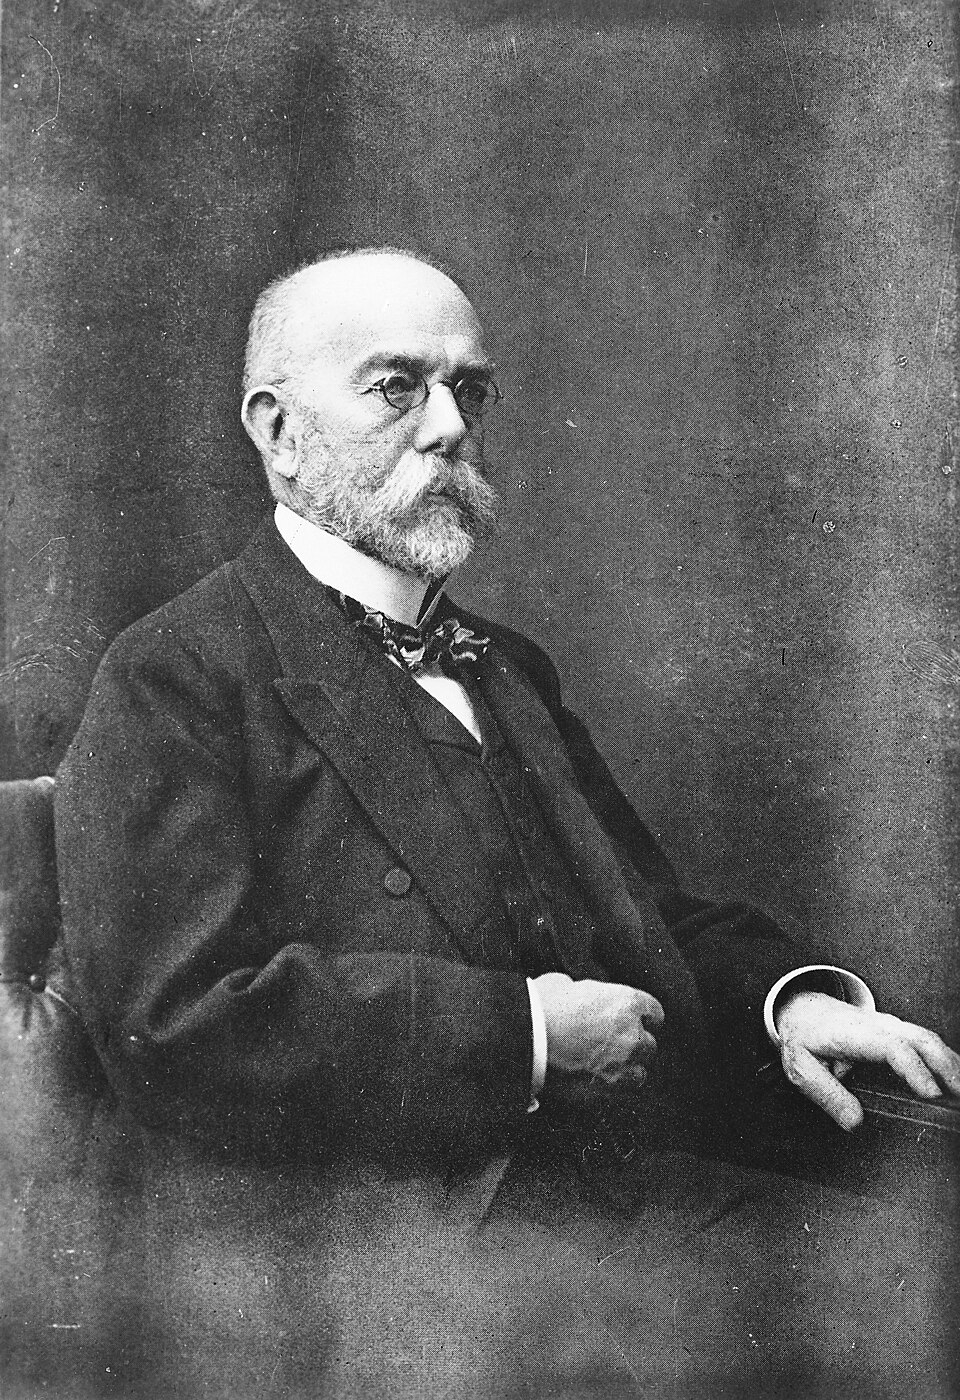
\includegraphics[width=0.30\linewidth]{images/book5/koch.jpg}\hspace{0.04\linewidth}
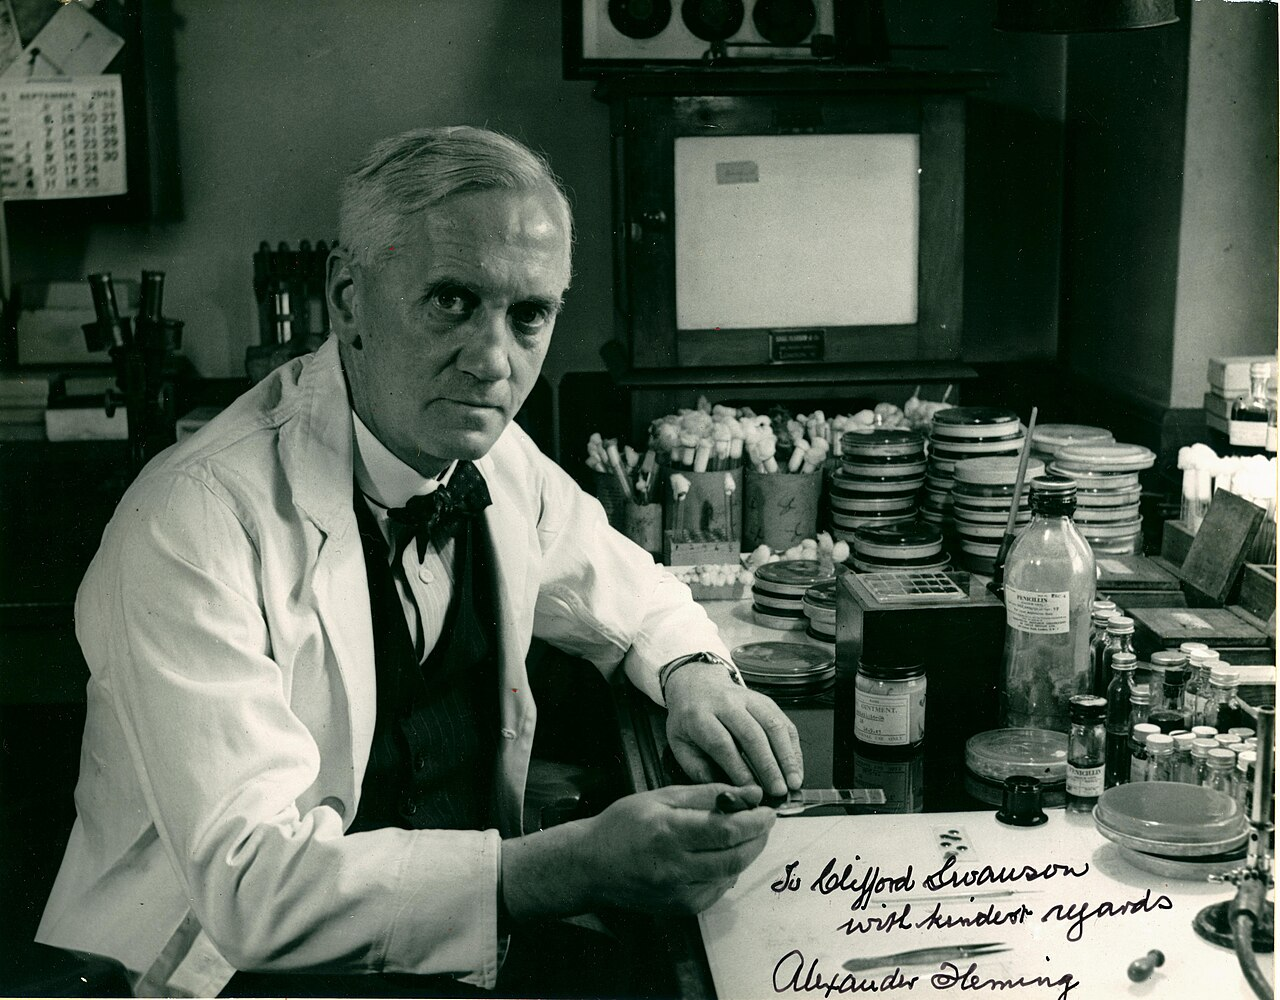
\includegraphics[width=0.56\linewidth]{images/book5/fleming.jpg}

{\small Robert Koch, que demostró que bacterias concretas causan
enfermedades concretas e inventó los métodos para cultivarlas (Wellcome
Collection, CC~BY~4.0). Derecha: Alexander Fleming en su laboratorio con
placas del moho cuyo producto llegó a ser la penicilina (archivo de la
Armada de los EE.\,UU., dominio público).}
\end{omfigure}

\section{Antibióticos y resistencia}

\begin{definition}[Antibióticos]\label{def:b3:bacteriology:antibiotics}
\index{antibiótico}\index{betalactámico}\index{toxicidad selectiva}\index{concentración mínima inhibitoria}
Un \emph{antibiótico} es una molécula que mata bacterias o detiene su
crecimiento a concentraciones inocuas para el hospedador, actuando sobre
una diana que el hospedador no tiene o tiene en otra forma --- la
\emph{toxicidad selectiva}. Las dianas son pocas. La pared celular: los
\emph{$\beta$-lactámicos} (penicilinas, cefalosporinas, carbapenémicos)
imitan el D-Ala-D-Ala terminal del péptido del \omterm{def:b3:bacteriology:envelope}{peptidoglicano} y acilan a
las enzimas que lo entrecruzan, de modo que la pared en crecimiento es
débil y la célula estalla por su propia turgencia; la vancomicina une el
propio D-Ala-D-Ala. El ribosoma, cuya forma bacteriana difiere de la
eucariota: los aminoglicósidos (la subunidad pequeña, con lecturas
erróneas), las tetraciclinas (que bloquean la entrada del ARNt), los
macrólidos y el cloranfenicol (el túnel de salida y la
peptidil-transferasa de la subunidad grande). La ADN-girasa y la
topoisomerasa~IV: las quinolonas. La ARN-polimerasa: la rifampicina. La
síntesis de folato, que los animales no hacen: las sulfamidas y el
trimetoprim. La membrana: las polimixinas, último recurso. La
\emph{concentración mínima inhibitoria} (CMI) es la concentración más
baja de un fármaco que impide el crecimiento visible de una cepa; una
cepa se llama resistente cuando su CMI supera la concentración que el
fármaco alcanza en el paciente.
\end{definition}

\begin{method}[Medir la sensibilidad]\label{met:b3:bacteriology:mic}
\index{difusión en disco}\index{dilución en caldo}
Dos pruebas. La \emph{\omterm{met:b3:bacteriology:mic}{dilución en caldo}}: inocúlese un número fijo de
células (unas $5\times 10^{5}$ por mililitro) en una fila de tubos o
pocillos con el \omterm{def:b3:bacteriology:antibiotics}{antibiótico} en pasos dobles, incúbese toda la noche y
léase el primer pocillo transparente: esa concentración es la CMI. La
\emph{\omterm{met:b3:bacteriology:mic}{difusión en disco}}: extiéndase la cepa en una placa de agar,
colóquense discos de papel cargados con cantidades conocidas de varios
\omterm{def:b3:bacteriology:antibiotics}{antibióticos} e incúbese; el fármaco difunde hacia fuera y su
concentración cae con la distancia, y el crecimiento queda inhibido hasta
el radio en el que la concentración iguala a la CMI, de modo que el
diámetro del halo claro --- leído en tablas calibradas --- da la
sensibilidad a cada disco en una sola placa. Ambas pruebas duran un día;
secuenciar el genoma en busca de genes y mutaciones de resistencia
conocidos cuesta lo mismo y empieza a sustituirlas.
\end{method}

\begin{definition}[Resistencia]\label{def:b3:bacteriology:resistance}
\index{resistencia a antibióticos}\index{betalactamasa}\index{bomba de expulsión}\index{SARM}
Una bacteria resiste a un \omterm{def:b3:bacteriology:antibiotics}{antibiótico} por uno de cinco medios. Destruye
el fármaco: las \emph{$\beta$-lactamasas} hidrolizan el anillo
$\beta$-lactámico,
y las variantes de espectro extendido y las carbapenemasas destruyen hoy
las más nuevas. Altera la diana: una mutación de la proteína ribosómica o
de la girasa que el fármaco une o, en el SARM (\emph{Staphylococcus
aureus} resistente a la meticilina), un gen adquirido de una enzima de
entrecruzamiento a la que los $\beta$-lactámicos no se unen; la
resistencia a
la vancomicina sustituye el D-Ala terminal por D-lactato, que el fármaco
no reconoce. Expulsa el fármaco con \emph{bombas de expulsión}, a menudo
de amplia especificidad. Impide que el fármaco entre, perdiendo una
porina. O sortea el paso bloqueado con una enzima alternativa. Las
mutaciones de la diana surgen por azar en el paciente a velocidades de
$10^{-8}$ a $10^{-6}$ por división y se seleccionan durante el
tratamiento; las enzimas y las bombas se adquieren en su mayoría en
\omterm{def:b3:genetic-engineering:tools}{plásmidos} del inmenso reservorio de bacterias del suelo y del intestino,
en el que evolucionaron durante eras frente a los \omterm{def:b3:bacteriology:antibiotics}{antibióticos} que
fabrican los hongos y otras bacterias. Las persistentes --- células
latentes que sobreviven a un fármaco sin ser genéticamente resistentes
--- explican las recaídas tras tratamientos que deberían haber
funcionado.
\end{definition}

\begin{proposition}[Por qué la resistencia es inevitable y la combinación es la respuesta]\label{prop:b3:bacteriology:selection}
\index{resistencia!selección}\index{terapia combinada!antibióticos}
Una infección de $10^{9}$ células tratada con un fármaco frente al que
las mutaciones de resistencia surgen a $10^{-8}$ por división ya contiene
unas diez células resistentes; el fármaco mata a las demás y las diez se
adueñan del terreno --- la aritmética del \cref{ch:b3:cancer-biology} sin
más, ya que una población bacteriana y un \omterm{def:b3:cancer-biology:hallmarks}{tumor} son ambos clones que
evolucionan bajo selección. Dos fármacos de dianas independientes se
enfrentan a una célula doblemente resistente a $10^{-16}$ por división,
que mil millones de células no contienen. Es por esto por lo que la
tuberculosis, cuyas lesiones albergan de $10^{8}$ a $10^{9}$ bacilos, se
trata con tres o cuatro fármacos a la vez desde los años cincuenta y por
lo que su monoterapia producía resistencia en cuestión de meses; y es
también por lo que todo uso de un \omterm{def:b3:bacteriology:antibiotics}{antibiótico}, en un paciente o en un
cebadero, selecciona resistencia en algún sitio, y por lo que el ritmo de
aparición de \omterm{def:b3:bacteriology:antibiotics}{antibióticos} nuevos --- ninguno de clase nueva contra las
\omterm{def:b3:bacteriology:envelope}{gramnegativas} desde los años sesenta --- es la medida frente a la que se
cuentan las pérdidas. Los remedios son los de cualquier contienda
evolutiva: usar menos, combinar, terminar el tratamiento para que las
células parcialmente resistentes no sobrevivan para reproducirse, y
buscar dianas nuevas.
\end{proposition}

\begin{example}[La ventana de selección de mutantes]\label{ex:b3:bacteriology:window}
Una cepa tiene una CMI de \qty{1}{mg/L}; sus mutantes resistentes de
primer paso, presentes a razón de uno de cada $10^{7}$, tienen una CMI de
\qty{8}{mg/L}. Una dosis que mantenga el fármaco en \qty{4}{mg/L} mata al
tipo silvestre y deja a los mutantes crecer sin competencia: el intervalo
de concentraciones entre la CMI del tipo silvestre y la de los mutantes
es la \emph{ventana de selección de mutantes}, y un tratamiento que se
quede dentro de ella cría resistencia. Una dosis por encima de
\qty{8}{mg/L} mata a los dos; una dosis demasiado baja, o un tratamiento
interrumpido cuando el paciente se encuentra mejor y el nivel del fármaco
está bajando por la ventana, es como se fabrica una población resistente.
La misma lógica fija las pautas del tratamiento de la tuberculosis: seis
meses, cuatro fármacos y dosis por encima de la CMI de todo mutante de un
solo paso.
\end{example}

\begin{omfigure}
\begin{tikzpicture}
\begin{axis}[
  width=0.7\linewidth, height=5.6cm,
  axis x line=bottom, axis y line=left,
  xmin=0, xmax=24, ymin=0.25, ymax=32, ymode=log,
  xlabel={horas tras una dosis}, ylabel={fármaco en plasma (mg/L)},
  xlabel style={font=\small, at={(axis description cs:0.5,-0.12)}, anchor=north}, ylabel style={font=\small},
  tick label style={font=\small}, xtick={0,6,12,18,24}, ytick={0.5,1,2,4,8,16}, yticklabels={0.5,1,2,4,8,16},
  clip=false,
]
\fill[omThm!15] (axis cs:0,1) rectangle (axis cs:24,8);
\addplot[very thick, omDef, domain=0:24, samples=60] {16*exp(-0.15*x)};
\addplot[dashed, gray, domain=0:24, samples=2] {1}; \addplot[dashed, gray, domain=0:24, samples=2] {8};
\node[font=\scriptsize, gray, anchor=south west] at (axis cs:0.3,1.05) {CMI del tipo silvestre};
\node[font=\scriptsize, gray, anchor=south east] at (axis cs:23.7,8.4) {CMI del mutante de primer paso};
\node[font=\scriptsize, omThm!70!black, anchor=west] at (axis cs:13,3.5) {ventana de selección de mutantes};
\node[font=\scriptsize, omDef, anchor=south west] at (axis cs:2,13) {nivel plasmático tras una dosis};
\end{axis}
\end{tikzpicture}

{\small La ventana de selección de mutantes. Un nivel de fármaco por
encima de la CMI de los mutantes lo mata todo; entre las dos CMI (zona
sombreada) mata al tipo silvestre y selecciona a los mutantes. Una dosis
cuyo nivel cae por la ventana durante horas, o un tratamiento
interrumpido antes de tiempo, cría resistencia.}
\end{omfigure}

\begin{remark}[La mayoría de las bacterias no son patógenas]\label{rem:b3:bacteriology:most}
Las bacterias de la clínica de este capítulo son una minoría minúscula.
Del millón de especies estimadas, unos pocos centenares causan enfermedad
humana; el resto llevan los ciclos del nitrógeno, del azufre y del
carbono (el volumen de segundo año), fijan el nitrógeno de todas las
leguminosas, digieren la celulosa de todos los rumiantes y componen los
microbiomas del \cref{ch:b3:microbiomes}, cuya pérdida bajo un
tratamiento \omterm{def:b3:bacteriology:antibiotics}{antibiótico} es un coste de cada tanda. Los propios
\omterm{def:b3:bacteriology:antibiotics}{antibióticos} son moléculas suyas --- armas y señales que evolucionaron
entre bacterias del suelo y hongos mucho antes de que hubiera hospitales
--- y también lo son casi todos los genes de resistencia.
\end{remark}

\section{Ejercicios}

\begin{exercise}[$\star$]\label{exo:b3:bacteriology:1}
Descríbanse las envolturas \omterm{def:b3:bacteriology:envelope}{grampositiva} y \omterm{def:b3:bacteriology:envelope}{gramnegativa} y explíquese por
qué la \omterm{met:b3:bacteriology:gram}{tinción de Gram} las distingue.
\end{exercise}

\begin{exercise}[$\star$]\label{exo:b3:bacteriology:2}
Un cultivo de $10^{3}$ células por mililitro llega a $10^{9}$ en
\qty{8}{h} de crecimiento exponencial. Hállense el número de
generaciones, el tiempo de generación y $\mu$.
\end{exercise}

\begin{exercise}[$\star$]\label{exo:b3:bacteriology:3}
Nómbrense las tres rutas de la transferencia horizontal de genes y dese
el experimento clásico que demostró cada una.
\end{exercise}

\begin{exercise}[$\star$]\label{exo:b3:bacteriology:4}
Dense la diana de la penicilina, de la estreptomicina, del
ciprofloxacino y de la rifampicina, y dígase por qué cada una es
selectivamente tóxica.
\end{exercise}

\begin{exercise}[$\star\star$]\label{exo:b3:bacteriology:5}
Un quimiostato tiene $\mu_{\max} = \qty{0.8}{h^{-1}}$, $K_{S} =
\qty{0.02}{g/L}$, $S_{0} = \qty{2}{g/L}$, $Y = 0.4$. Calcúlense $S^{*}$ y
$X^{*}$ en $D = 0.2$, $0.6$ y $0.79$ h$^{-1}$, y la \omterm{thm:b3:bacteriology:monod}{tasa de dilución} a la
que empieza el arrastre.
\end{exercise}

\begin{exercise}[$\star\star$]\label{exo:b3:bacteriology:6}
Con la \cref{prop:b3:bacteriology:threshold}, compárese la densidad
umbral de la \omterm{def:b3:bacteriology:quorum}{percepción de quórum} en un órgano luminoso de calamar ($k =
\qty{0.01}{h^{-1}}$) y en agua de mar en movimiento ($k = \qty{10}{h^{-1}}$),
con $p = 100$ moléculas por célula y hora y $A_{\text{umbr}} =
\qty{10}{nmol/L}$ ($6\times 10^{12}$ moléculas por litro).
\end{exercise}

\begin{exercise}[$\star\star$]\label{exo:b3:bacteriology:7}
Una placa de \omterm{met:b3:bacteriology:mic}{difusión en disco} muestra halos de $25$, $12$ y
\qty{0}{mm} para tres fármacos. Interprétese cada uno y explíquese por
qué un diámetro de halo puede convertirse en una CMI.
\end{exercise}

\begin{exercise}[$\star\star$]\label{exo:b3:bacteriology:8}
Explíquese cómo un solo suceso de \omterm{def:b3:bacteriology:hgt}{conjugación} puede hacer resistente a
cinco \omterm{def:b3:bacteriology:antibiotics}{antibióticos} a una \emph{Klebsiella} sensible, y por qué los genes
de resistencia se encuentran tan a menudo juntos en \omterm{def:b3:genetic-engineering:tools}{plásmidos}.
\end{exercise}

\begin{exercise}[$\star\star$]\label{exo:b3:bacteriology:9}
Un paciente tiene $10^{9}$ bacterias y toma un fármaco frente al que la
resistencia surge a $10^{-7}$ por división. Calcúlense las células
resistentes esperadas al inicio; después, con dos fármacos
independientes. ¿Por qué las persistentes son otro problema?
\end{exercise}

\begin{exercise}[$\star\star\star$]\label{exo:b3:bacteriology:10}
Muéstrese que el estado estacionario del quimiostato es estable:
pertúrbese $X$ ligeramente por encima de $X^{*}$ y sígase el signo de
$\mathrm{d}S/\mathrm{d}t$ y de $\mathrm{d}X/\mathrm{d}t$. Explíquese
después por qué dos especies que compiten por un nutriente en un
quimiostato no pueden coexistir en el estado estacionario, y cuál gana a
un $D$ dado.
\end{exercise}

\begin{exercise}[$\star\star\star$]\label{exo:b3:bacteriology:11}
El \omterm{def:b3:bacteriology:quorum}{autoinductor} induce su propia sintasa. Modifíquese el modelo de la
\cref{prop:b3:bacteriology:threshold} de modo que $p$ salte de $p_{0}$ a
$p_{1} \gg p_{0}$ cuando $A > A_{\text{umbr}}$, y muéstrese que el sistema
puede tener dos estados estables en un intervalo de densidades (la
histéresis): una población que se ha encendido sigue encendida a una
densidad en la que una población ingenua estaría apagada. ¿Cuál es la
utilidad biológica de eso?
\end{exercise}

\begin{exercise}[$\star\star\star$]\label{exo:b3:bacteriology:12}
Explíquese la ventana de selección de mutantes y úsese para argumentar a
favor o en contra de cada cosa: (a) dosis altas en tandas cortas;
(b) dosis bajas en tandas largas; (c) interrumpir cuando ceden los
síntomas; (d) la \omterm{thm:b3:cancer-biology:goldie-coldman}{terapia combinada}.
\end{exercise}

\section{Problema: un quimiostato y una clínica}

\begin{problem}[{Problema de fin de semana --- un cultivo crecido en un
matraz y mantenido en un quimiostato, una bacteria luminosa contada hasta
su quórum y una infección tratada frente a la aritmética de la
resistencia, hasta llegar a las células del quimiostato, a la densidad a
la que se enciende la luz y a las probabilidades de que una tanda de dos
fármacos encuentre una célula resistente}]
\label{pb:b3:bacteriology:1}
Datos: \emph{E.~coli} a \qty{37}{\celsius}, $T = \qty{20}{min}$; una
célula pesa \qty{1}{pg}. Quimiostato: $V = \qty{1}{L}$,
$F = \qty{0.5}{L/h}$, $\mu_{\max} = \qty{1.0}{h^{-1}}$,
$K_{S} = \qty{0.01}{g/L}$, $S_{0} =
\qty{2}{g/L}$ de glucosa, $Y = 0.5$. \emph{Vibrio}: $p = 500$ moléculas
de \omterm{def:b3:bacteriology:quorum}{autoinductor} por célula y hora, $A_{\text{umbr}} = 6\times 10^{12}$
moléculas por litro (\qty{10}{nmol/L}), $k = \qty{0.05}{h^{-1}}$ en el
órgano luminoso. Infección: $10^{9}$ células; resistencia al fármaco A a
$10^{-8}$ por división y al fármaco B a $10^{-7}$; CMI del tipo silvestre
para A, \qty{1}{mg/L}, y del mutante de primer paso, \qty{8}{mg/L}; una
dosis da \qty{16}{mg/L} que cae con semivida \qty{4}{h}.

\medskip
\noindent\textbf{Parte I --- El matraz.}
\begin{enumerate}
  \item Una célula en \qty{100}{mL} de caldo. ¿Cuántas células al cabo
        de \qty{6}{h} de crecimiento exponencial, y qué densidad por mL?
  \item El caldo sostiene como mucho $2\times 10^{9}$ células por mL.
        ¿Cuándo se detiene el crecimiento, y cuál es la masa de células
        del cultivo?
  \item ¿Cuánto tardarían los descendientes de una célula en alcanzar la
        masa de la Tierra ($6\times 10^{27}$ g)? Coméntese.
  \item La \omterm{def:b3:bacteriology:phases}{fase de latencia} dura \qty{1}{h} cuando se inoculan en medio
        fresco células de la \omterm{def:b3:bacteriology:phases}{fase estacionaria}, y casi nada cuando se
        usan células en fase exponencial. Explíquese.
  \item Calcúlese $\mu$ a partir de $T$. Si se cambia el medio a un
        azúcar en el que $T = \qty{60}{min}$, ¿cuál es $\mu$, y por qué
        factor cae el número de células al cabo de \qty{6}{h}?
  \item Una muestra del cultivo estacionario se extiende en una placa y
        da $200$ colonias a partir de \qty{0.1}{mL} de una dilución
        $10^{-6}$. ¿Cuál es el recuento de viables, y por qué podría
        diferir de un recuento al microscopio?
\end{enumerate}

\medskip
\noindent\textbf{Parte II --- El quimiostato.}
\begin{enumerate}[resume]
  \item Calcúlense la \omterm{thm:b3:bacteriology:monod}{tasa de dilución} $D$ y el tiempo de generación que
        el cultivo se ve obligado a adoptar.
  \item Calcúlense $S^{*}$ y $X^{*}$ (en g/L y en células por mL).
  \item ¿Cuántas células salen del recipiente por hora? ¿Cuántas
        generaciones recorre el cultivo en un mes?
  \item La bomba se sube a $F = \qty{0.95}{L/h}$. ¿Nuevos $S^{*}$ y
        $X^{*}$? ¿Qué ocurre con $F = \qty{1.1}{L/h}$?
  \item Aparece un mutante con $\mu_{\max} = \qty{1.2}{h^{-1}}$ y el
        mismo $K_{S}$. Con $D = 0.5$, ¿qué $S^{*}$ necesita, y qué le
        ocurre a la cepa original? (Úsese el
        \cref{exo:b3:bacteriology:10}.)
  \item Un mes de funcionamiento son $700$ generaciones. Si una mutación
        beneficiosa surge a $10^{-9}$ por división y el recipiente
        contiene $10^{12}$ células, ¿cuántas mutaciones beneficiosas
        surgen por generación? ¿Qué dice esto sobre la evolución en un
        quimiostato?
\end{enumerate}

\medskip
\noindent\textbf{Parte III --- El quórum.}
\begin{enumerate}[resume]
  \item Calcúlese la densidad celular umbral para la luz en el órgano
        luminoso, en células por mL.
  \item El órgano luminoso contiene \qty{1}{\micro L} de bacterias a
        $10^{10}$ por mL. ¿Por qué factor supera el \omterm{def:b3:bacteriology:quorum}{autoinductor} al
        umbral?
  \item En el agua de mar la señal se la lleva la corriente con
        $k = \qty{20}{h^{-1}}$. ¿Densidad umbral? Compárese con las
        $10^{2}$ células por mL de mar abierto.
  \item Después de que el calamar expulse el \qty{90}{\%} de las
        bacterias al amanecer, ¿cuánto tardan las $10^{9}$ por mL
        restantes, que se dividen cada \qty{2}{h}, en restaurar $10^{10}$
        por mL? ¿Se apaga la luz entretanto?
  \item Cada célula que brilla gasta alrededor del \qty{20}{\%} de su
        energía en la luz. ¿Por qué se ve favorecida una célula oscura en
        el mar, y por qué no en el órgano?
  \item Un patógeno usa el mismo sistema para retrasar sus toxinas hasta
        ser numeroso. Propóngase una estrategia farmacológica que
        aproveche esto y dígase por qué podría seleccionar resistencia
        más despacio que un \omterm{def:b3:bacteriology:antibiotics}{antibiótico}.
\end{enumerate}

\medskip
\noindent\textbf{Parte IV --- La clínica.}
\begin{enumerate}[resume]
  \item Número esperado de células resistentes a A al empezar el
        tratamiento; a B; a ambos.
  \item Probabilidad de que no exista ninguna célula resistente a A; y a
        ambos.
  \item Tras la dosis, ¿cuándo baja el nivel del fármaco a
        \qty{8}{mg/L}, y a \qty{1}{mg/L}? ¿Cuánto tiempo pasa por dosis
        dentro de la ventana de selección de mutantes?
  \item Si el fármaco se administra cada \qty{12}{h}, ¿qué fracción del
        tiempo está el nivel dentro de la ventana, y qué predice eso a lo
        largo de una tanda de diez días solo con A?
  \item Propóngase un cambio de pauta que mantenga el nivel por encima de
        \qty{8}{mg/L} en todo momento (calcúlese el intervalo o la dosis
        necesarios), y enúnciese su coste.
  \item Una célula de cada $10^{4}$ es persistente, latente e intocable
        por cualquier concentración de ninguno de los dos fármacos.
        ¿Cuántas sobreviven a la tanda, qué ocurre cuando se retira el
        fármaco y qué implica esto para la duración del tratamiento?
  \item Resúmase: las células por mL del quimiostato (pregunta~8), la
        densidad umbral de la luz (pregunta~13) y la probabilidad de que
        la tanda de dos fármacos no encuentre ninguna célula resistente
        (pregunta~20).
\end{enumerate}
\end{problem}
